\documentclass[12pt,a4paper,oneside]{report}
\usepackage[margin=27mm,headheight=15pt]{geometry}
\usepackage{fontspec}
\setmainfont{TeX Gyre Pagella}
\setsansfont{TeX Gyre Heros}
\setmonofont{DejaVu Sans Mono}[Scale=0.82]
\usepackage{amsmath,amssymb,amsthm,mathtools,booktabs,longtable,array,graphicx,caption,enumitem}
\usepackage{microtype,tikz,pgfplots,hyperref,bookmark,fancyhdr,listings,xcolor}
\usetikzlibrary{positioning}
\pgfplotsset{compat=1.18}
\hypersetup{colorlinks=true,linkcolor=black,citecolor=black,urlcolor=blue,pdftitle={Prompt Engineering as a Discrete-Continuous Optimization Problem},pdfauthor={Charalampos Nadiotis}}
\pagestyle{fancy}\fancyhf{}\fancyhead[L]{\small Prompt Engineering: Discrete-Continuous Optimization}\fancyhead[R]{\small BSc Research Draft}\fancyfoot[C]{\thepage}
\newtheorem{theorem}{Theorem}[chapter]
\newtheorem{proposition}[theorem]{Proposition}
\newtheorem{definition}[theorem]{Definition}
\newtheorem{remark}[theorem]{Remark}
\newcommand{\Vocab}{\mathcal V}
\newcommand{\Pspace}{\mathcal P}
\newcommand{\R}{\mathbb R}
\newcommand{\E}{\mathbb E}
\newcommand{\ind}{\mathbb I}
\newcommand{\sig}{\sigma}
\lstset{basicstyle=\ttfamily\scriptsize,breaklines=true,frame=single,columns=fullflexible,showstringspaces=false}
\begin{document}
\begin{titlepage}
\centering
{\Large Frederick University\par}\vspace{7mm}
{\large Department of Computer Science\par}\vspace{30mm}
{\Huge\bfseries Prompt Engineering as a\par}
\vspace{4mm}{\Huge\bfseries Discrete-Continuous\par}
\vspace{4mm}{\Huge\bfseries Optimization Problem\par}
\vspace{12mm}
{\Large A Mathematical Perspective Using Discrete Mathematics, Calculus and Reproducible Evaluation\par}
\vspace{24mm}
{\Large Bachelor's Thesis - Working Dissertation\par}
\vspace{13mm}
{\Large Charalampos Nadiotis\par}
\vfill
{\large Academic supervisor: Dr. Stephania Loizidou\par}
\vspace{2mm}
{\large Nicosia, Cyprus - Draft prepared November 2026 for January 2027\par}
\vspace{13mm}
\begin{minipage}{0.84\linewidth}\centering\small
\textbf{Evidence status:} The theoretical argument and deterministic synthetic experiments are documented and reproducible. Actual large-language-model evaluation, departmental approval and any human-participant study have not yet been completed. This document is not represented as a final accepted dissertation.
\end{minipage}
\end{titlepage}
\pagenumbering{roman}
\chapter*{Abstract}
\addcontentsline{toc}{chapter}{Abstract}
A textual prompt is an ordered sequence of symbols from a finite vocabulary, whereas its evaluation by a neural language model is mediated by vectors, matrices, nonlinear functions and probability distributions. This dissertation examines prompt engineering at the interface between discrete combinatorial search and continuous computation. It extends the author's submitted October 2026 article of the same title into a mathematical and experimental investigation. The theoretical component defines a constrained prompt-search objective, reviews the derivatives governing attention-related and soft-prompt operations, derives a sensitivity bound for a differentiable scoring surrogate, and proves exact finite-search expressions for random-search success and expected best score. The implementation component provides a dependency-free Python benchmark with a six-token abstract vocabulary, two-dimensional embeddings and a set of fixed synthetic task vectors. Exact enumeration establishes the optimum for prompt lengths two, three and four. Random search and restarting first-improvement coordinate search are compared under identical counts of objective evaluations across twelve budget-length configurations, with fifty deterministic seeds each. Twenty-seven local automated tests verify mathematical identities, exhaustive enumeration, reproducibility, evaluation budgets, per-state gradient ranking, discrete stopping points and an offline results-scoring interface. A representative three-token, thirty-six-call configuration yields mean synthetic scores of 0.745721 and 0.746977 for random and coordinate search, respectively, versus the exact optimum of 0.747292. These outcomes demonstrate properties of the stated surrogate, \emph{not} improved prompting of a deployed LLM. A prospective held-out real-model evaluation protocol is defined but not claimed to have been executed. The thesis contributes a transparent bridge between mathematical abstraction, reproducible finite optimization and the evidence requirements of future empirical prompt-engineering research.

\noindent\textbf{Keywords:} prompt engineering, discrete optimization, calculus, embeddings, finite search, reproducibility, synthetic benchmark, large language models.
\clearpage
\chapter*{Research integrity and evidence declaration}
\addcontentsline{toc}{chapter}{Research integrity and evidence declaration}
The dissertation builds on the author's article \emph{Prompt Engineering as a Discrete-Continuous Optimization Problem: A Mathematical Perspective Using Discrete Mathematics and Calculus}, dated October 2026 and described by the author as submitted. The article presents theory and literature synthesis, it does not claim to report a completed LLM experiment. All synthetic data, model parameters and evaluation methods used in this dissertation are fully specified in the accompanying source code. A score such as 0.746977 is \emph{not} accuracy, human preference, benchmark performance or a result from an actual language model. No human subjects, paid APIs or proprietary models were used for this executable milestone. Reproducibility statements describe the checked local environment and do not imply independent replication or supervisor approval. The manuscript retains placeholders where the university's exact title-page, ethics and assessment requirements have not been supplied.
\tableofcontents
\listoftables
\listoffigures
\clearpage
\pagenumbering{arabic}

\chapter{Introduction}
\section{The research problem}
For conventional software, the programmer usually specifies explicit operations in a programming language. For a large language model (LLM), a user often alters a text instruction, demonstration sequence or output constraint to influence a learned probabilistic system. The formal domain of selectable instructions is finite at any fixed token length, but the computations induced by those instructions live in continuous vector spaces. Confusing these two domains can lead to inaccurate claims: a textual edit is not infinitesimal, a derivative of the network is not a derivative with respect to a word, and a well-performing prompt on one dataset does not automatically transfer to another model or dataset.

The author's submitted article identified this discrete-continuous duality. This dissertation develops it into a testable research programme while holding the evidentiary boundary between theory, synthetic experiment and LLM evaluation. The issue is not merely whether optimization methods can find a useful string, but \emph{what} has been optimized, under which scoring function, at what evaluation cost, and what conclusions the results support.

\section{Research objectives and questions}
The objectives are (i) to provide a consistent mathematical representation, (ii) to derive checkable properties of finite prompt search and continuous score sensitivity, (iii) to implement budget-controlled comparison methods, and (iv) to specify tests needed for a defensible future LLM study.

\begin{description}[leftmargin=20mm,style=nextline]
\item[RQ1.] How can prompt selection and differentiable embedding-space computation be written in one constrained optimization model?
\item[RQ2.] Which quantitative results - counting, derivatives, best-of-budget statistics and regret - can be established without running an LLM?
\item[RQ3.] Under identical score-call budgets, how do random and coordinate-based search behave on the specified finite surrogate?
\item[RQ4.] Which data, controls and reporting conventions would be required to extend these methods to real language models?
\end{description}

\section{Contributions and their limits}
The completed contributions are a mathematical formulation, two analytic results for finite search, a sensitivity bound, open executable benchmark code, exhaustive oracles for three prompt lengths, independent held-out synthetic scores, generated result tables, and twenty-two automated tests. These contributions constitute an undergraduate-scale computational study. They are not a new transformer architecture, a proof about general LLM performance, a new universal prompt-search algorithm or a validated cognitive theory of language instruction.

\section{Organization}
Chapter 2 surveys the main research families. Chapter 3 introduces the mathematical setting. Chapter 4 derives finite-search results and sensitivity properties. Chapter 5 describes the experiment and software. Chapter 6 reports measured surrogate results. Chapter 7 documents MATLAB-ready graphics and audit boundaries. Chapter 8 develops a prospective real-model evaluation protocol. Chapter 9 discusses threats to validity. Chapter 10 gives conclusions and next actions. The appendices define the artifact structure, reproduction procedure and evidence register.

\chapter{Background and Related Work}
\section{Transformers and in-context conditioning}
Vaswani and colleagues established a transformer architecture based on attention mechanisms \cite{vaswani2017}. Brown and colleagues described few-shot language-model behavior in which examples are placed in the context rather than used for parameter updates \cite{brown2020}. These are relevant because the prompt influences the conditional distribution over output tokens while the deployed model parameters may be fixed. It does not follow that all prompt formats have equivalent effects.

For a prompt $p$ and task input $x$, an autoregressive model assigns
\begin{equation}
P_{\theta}(y\mid p,x)=\prod_{t=1}^{T}P_{\theta}(y_t\mid p,x,y_{<t}).
\label{eq:auto}
\end{equation}
Here $\theta$ denotes frozen model parameters. Inference can be deterministic or stochastic depending on decoding. A reproducible evaluation must record the decoding policy.

\section{Textual prompt search}
The systematic review of Liu and colleagues organizes prompt-based learning approaches and their design space \cite{liu2023}. Automatic Prompt Engineer treats instructions as generated candidates evaluated against a score \cite{zhou2023}. The gradient-guided AutoPrompt method uses differentiable information to suggest discrete token replacements \cite{shin2020}. These methods have different assumptions about gradients, candidate proposals and model access, they should not be grouped into a single empirical baseline without normalization.

\section{Example choice and ordering}
Given $n$ demonstrations and $k$ available positions, selecting ordered examples without replacement produces $n!/(n-k)!$ candidate lists. Empirical work by Lu and colleagues shows that prompt order can materially alter few-shot performance \cite{lu2022}, Zhao and colleagues investigate calibration and sensitivity to prompt design \cite{zhao2021}. The combinatorial count explains the size of the design space but not which ordering works on a particular task.

\section{Soft prompts and continuous optimization}
Lester and colleagues study learned, continuous prompt vectors while keeping the underlying model frozen \cite{lester2021}. Unlike ordinary vocabulary tokens, these vectors admit infinitesimal perturbations and gradient updates. Prompt tuning therefore provides a concrete example of continuous optimization at the input interface. The present benchmark does not train a soft prompt and cannot reproduce those results, it uses a deliberately smaller differentiable function to validate the mathematical bridge.

\section{Gap addressed by this dissertation}
A great deal of prior work evaluates effective prompting techniques using actual models. This thesis takes a narrower methodological role: it constructs an exact, finite reference problem whose optimization and measurement properties can be independently checked. Its value lies in transparent accounting for oracle optima, score calls, random-search expectations and evidence limitations. Such a benchmark is a validation stage, not an alternative to real-model experiments.

\chapter{Mathematical Foundations}
\section{Discrete prompt representations}
\begin{definition}[Finite textual prompt]
Let $\Vocab$ be a finite vocabulary of cardinality $N$. A length-$m$ prompt is an ordered tuple $p=(t_1,\dots,t_m)\in\Vocab^m$. A feasible subset $\Pspace\subseteq\bigcup_{m=1}^{L}\Vocab^m$ may impose syntax, length and cost constraints.
\end{definition}
For a fixed length, the search-space cardinality is
\begin{equation}|\Vocab^m|=N^m.\label{eq:count}\end{equation}
For $N=6$, the lengths studied here have $36$, $216$ and $1296$ possibilities. The number $N^m$ is a cardinality, not a prediction of how many semantically distinct or natural-language prompts exist. With vocabulary sizes in the tens of thousands and longer prompts, enumeration is not a practical general method.

\section{Task objective and constrained optimization}
Let $D$ be an evaluation distribution, $f_{\theta}$ a fixed model and $R$ an application-specific reward. The idealized task objective is
\begin{equation}
J_D(p)=\E_{(x,y)\sim D}\bigl[R(f_{\theta}(p,x),y)\bigr],
\qquad p^*\in\operatorname*{arg\,max}_{p\in\Pspace}J_D(p).
\label{eq:objective}
\end{equation}
If $f_\theta$ is stochastic, $R$ should be interpreted as including output sampling or an expectation over that randomness. A more operational formulation is
\begin{equation}\max_{p\in\Pspace}J_D(p)\quad\text{subject to }\ell(p)\le L,\ C(p)\le B,\ V(p)\le\varepsilon,\end{equation}
where $\ell$ is length, $C$ evaluation cost and $V$ a violation rate. The constraints must be defined and measured, not inferred from the wording of instructions.

\section{From symbols to vectors}
A token embedding is a map $E:\Vocab\to\R^d$. The prompt matrix is
\begin{equation}X(p)=\begin{bmatrix}E(t_1)^\top\\\vdots\\E(t_m)^\top\end{bmatrix}\in\R^{m\times d}.\end{equation}
Attention computes a continuous transformation of projections $Q=XW_Q$, $K=XW_K$ and $V=XW_V$:
\begin{equation}\operatorname{Attention}(Q,K,V)=\operatorname{softmax}\left(\frac{QK^\top}{\sqrt{d_k}}\right)V.\label{eq:attn}\end{equation}
The mapping can be differentiable in its vector inputs without a meaningful infinitesimal operation on token identities. Replacing $t_i$ by $t'_i$ changes an entire embedding vector, its magnitude can be large in embedding space.

\begin{figure}[htbp]\centering
\begin{tikzpicture}[node distance=18mm, every node/.style={font=\small}, >=stealth]
\node[draw,rounded corners,minimum width=36mm,minimum height=13mm] (a) {token tuple $p\in\Vocab^m$};
\node[draw,rounded corners,right=of a,minimum width=34mm,minimum height=13mm] (b) {embedding $X(p)$};
\node[draw,rounded corners,right=of b,minimum width=34mm,minimum height=13mm] (c) {$f_\theta$, logits};
\draw[->,thick] (a) -- node[above,fill=white,inner sep=1pt]{lookup} (b);
\draw[->,thick] (b) -- node[above,fill=white,inner sep=1pt]{continuous} (c);
\node[below=14mm of b,draw,dashed,align=center,minimum width=48mm] (d) {choose another discrete tuple\\or optimize continuous vectors};
\draw[->,dashed] (d.west) -- ++(-13mm,0) |- (a.south);
\end{tikzpicture}
\caption{The mathematical separation between prompt selection and differentiable computation. This diagram is schematic and does not depict the experimental surrogate as an LLM.}\label{fig:interface}
\end{figure}

\section{Probability, cross-entropy and gradients}
Given logits $z_1,\ldots,z_N$, softmax assigns $p_i=e^{z_i}/\sum_j e^{z_j}$. For one-hot targets $y_i$,
\begin{equation}\mathcal L=-\sum_i y_i\log p_i,\qquad \frac{\partial\mathcal L}{\partial z_i}=p_i-y_i.\label{eq:softmaxgrad}\end{equation}
To see the derivative, write $\mathcal L=-\sum_i y_i z_i +\log\sum_j e^{z_j}$ and differentiate with respect to $z_i$, using $\sum_i y_i=1$. This calculation concerns numeric logits, not direct differentiation of a textual token.

A trainable soft prompt $P\in\R^{m\times d}$ can be optimized by
\begin{equation}P^{(r+1)}=P^{(r)}-\eta\nabla_P\mathcal L(P^{(r)}).\end{equation}
For a candidate discrete replacement with embeddings $e,e'$, a first-order approximation is
\begin{equation}\mathcal L(e')\approx\mathcal L(e)+\nabla_e\mathcal L(e)^\top(e'-e).\label{eq:taylor}\end{equation}
Because $(e'-e)$ may not be small, the approximation is a ranking heuristic, not a proof of improvement.

\section{The mixed domain}
When both discrete tokens $p_d$ and trainable vectors $p_c$ are used, the decision space is $\Vocab^m\times\R^{k\times d}$. The objective can be jointly written $J(p_d,p_c)$ even when a practical algorithm alternates discrete and continuous updates. This \emph{does not} imply convexity or the special algebraic properties of a mixed-integer linear program.

\chapter{Finite Search Theory and a Differentiable Surrogate}
\section{Explicit surrogate definition}
A mathematical benchmark should expose every source of numerical behavior. Here the alphabet contains exactly six abstract token labels and each label has a fixed vector in $\R^2$. These names are identifiers, they do not represent empirically learned meanings. For a prompt $p=(t_1,\dots,t_m)$ define
\begin{equation}
\mathbf x(p)=\frac{1}{m}\sum_{i=1}^{m}(1+0.1(i-1))E(t_i).
\label{eq:embedding}
\end{equation}
The small position-dependent coefficient makes ordering observable. For target vector $u$ define the two logits $z_1=2\mathbf x^\top u$ and $z_0=-\mathbf x^\top u$. The score is
\begin{equation}
s(p,u)=\frac{e^{z_1}}{e^{z_1}+e^{z_0}}=\sig(3\mathbf x(p)^\top u),\qquad \sig(z)=\frac{1}{1+e^{-z}}.
\label{eq:surrogate}
\end{equation}
For the four fixed development targets $T=\{u_1,\dots,u_4\}$,
\begin{equation}J_T(p)=\frac14\sum_{j=1}^{4}s(p,u_j).\label{eq:train}\end{equation}
A separate fixed collection $H$ is used only for held-out synthetic scoring after prompt selection. Both collections consist of \emph{manually chosen vectors}, not sample prompts, documents or model outputs. Their exact values are stored in the Python code.

\section{A calculus result}
\begin{proposition}[Gradient and global Lipschitz bound]
For the continuous extension $J_T(\mathbf x)=|T|^{-1}\sum_{u\in T}\sig(3\mathbf x^\top u)$,
\begin{equation}
\nabla_{\mathbf x}J_T(\mathbf x)=\frac{3}{|T|}\sum_{u\in T}\sig(3\mathbf x^\top u)\bigl[1-\sig(3\mathbf x^\top u)\bigr]u.
\label{eq:grad}
\end{equation}
In Euclidean norm, $J_T$ is globally Lipschitz with constant no greater than $L_T=\frac{3}{4|T|}\sum_{u\in T}\|u\|_2$.
\end{proposition}
\begin{proof}
The chain rule gives Equation~\eqref{eq:grad}, since $\sig'(z)=\sig(z)(1-\sig(z))$. For all real $z$, $0<\sig(z)(1-\sig(z))\le 1/4$. The triangle inequality yields $\|\nabla J_T(\mathbf x)\|_2\le L_T$. Integrating along the segment between arbitrary $\mathbf x,\mathbf x'$ proves $|J_T(\mathbf x)-J_T(\mathbf x')|\le L_T\|\mathbf x-\mathbf x'\|_2$.
\end{proof}
This is a bound for \emph{this} surrogate only. It is not a globally valid Lipschitz constant for a transformer, nor a guarantee that one word substitution produces a small output difference. The code tests the analytical gradient against finite differences at an off-grid point.

\section{Exact oracle and regret}
For an alphabet of $N$ symbols, the exact oracle evaluates all $N^m$ candidates and returns $J^*=\max_{p\in\Vocab^m}J_T(p)$. For a candidate $\hat p$ define simple regret
\begin{equation}r(\hat p)=J^*-J_T(\hat p)\ge0.\label{eq:regret}\end{equation}
The inequality holds by the definition of a maximum. It is not a probabilistic performance guarantee for the search algorithm.

\begin{proposition}[Enumeration cost]
If evaluating $J_T$ for a prompt of length $m$ with $K$ target vectors costs $\Theta(m+K)$ for fixed embedding dimension, full enumeration costs $\Theta(N^m(m+K))$ arithmetic work and $N^m$ score evaluations.
\end{proposition}
\begin{proof}
The oracle enumerates exactly $N^m$ tuples. For each tuple, embedding construction performs $m$ vector additions and target scoring performs $K$ dot products and sigmoid calls. Summation gives the stated cost.
\end{proof}

\section{Exact random-search predictions}
Let $M=N^m$ be the number of candidate tuples and suppose $k$ candidates attain the oracle optimum. Independent, uniform random search with replacement misses the optimal set on a single draw with probability $1-k/M$. Consequently, after $B$ evaluations,
\begin{equation}
\Pr(\text{at least one optimum by }B)=1-\left(1-\frac{k}{M}\right)^B.
\label{eq:success}
\end{equation}
This is an \emph{exact} probability under the stated sampling law, not an estimated test result. If all distinct objective scores are $v_1<\dots<v_q$ and $F(v_j)=M^{-1}|\{p:J_T(p)\le v_j\}|$ with $F(v_0)=0$, then the exact expected best score after $B$ independent draws is
\begin{equation}
\E[J_{\mathrm{best},B}]=\sum_{j=1}^{q}v_j\left[F(v_j)^B-F(v_{j-1})^B\right].
\label{eq:expectedbest}
\end{equation}
\begin{proof}[Explanation]
The event that the maximum sampled score equals $v_j$ has probability $F(v_j)^B-F(v_{j-1})^B$, since all $B$ draws must be at most $v_j$ but not all below $v_j$. Multiply these disjoint probabilities by their respective values and sum.
\end{proof}
These expressions provide a calibration target for the random baseline. Coordinate search is adaptive and does not satisfy the iid assumption.

\chapter{Implementation and Evaluation Methodology}
\section{Software architecture}
The reproducible code is divided into \texttt{src/experiment.py}, \texttt{src/make\_tables.py}, \texttt{src/score\_outputs.py}, and a \texttt{tests} directory. The surrogate experiment uses only the Python standard library, an explicit seed per trial, fixed numbers and deterministic tie-breaking. Data are exported to machine-readable CSV and JSON. All manuscript numerical tables are regenerated from the saved JSON, preventing manual transcription drift.

\section{Algorithms}
The three-token instance has $6^3=216$ possible candidates. Exact enumeration supplies an oracle, not a competitive budgeted baseline. The random baseline draws candidates uniformly with replacement. The coordinate method begins at a seeded random prompt, considers one-position token substitutions in a shuffled order, accepts the first strictly improving substitution, and restarts from a fresh random candidate after a full unsuccessful sweep. The algorithm retains the best candidate across restarts. Every call to the scoring function is counted, including initial states and repeated candidates. Both search methods consume \emph{exactly} the same number $B$ of evaluations, the objective does not give free evaluations to either method.

\begin{table}[htbp]\centering\small
\caption{Experiment design, fixed before reporting results.}\label{tab:design}
\begin{tabular}{ll}\toprule Factor&Configuration\\\midrule Alphabet&6 symbolic tokens with fixed two-dimensional vectors\\
Lengths&$m\in\{2,3,4\}$\\
Budget (score calls)&$B\in\{12,24,36,72\}$\\
Randomization&seeds $0,1,\dots,49$ for each method and condition\\
Heuristics&uniform random, restarting first-improvement coordinate\\
Oracle&full enumeration at each prompt length\\
Development objectives&four fixed synthetic target vectors\\
Held-out objectives&four different, fixed synthetic target vectors\\
Primary outcome&mean simple regret from the train-set oracle\\
Secondary outcomes&held-out score, optimal hits, distinct candidates\\\bottomrule\end{tabular}
\end{table}

\section{Comparison logic}
All score-call budgets are matched, but a score call is not equivalent to identical wall-clock cost: neighbor generation and restart logic differ. Random search can revisit a tuple, coordinate search can do so too. Recording distinct candidates makes repeat sampling visible instead of silently treating budget as the number of unique prompts. Reported point estimates are arithmetic means over fifty fixed seeds. Percentile bootstrap intervals for mean regret are computed by resampling those fifty trials with a fixed bootstrap seed and 2000 replicates. They describe variation across these randomized starts and \emph{do not} quantify a population of real language-model tasks.

\section{Verification strategy}
Unit tests check stable logistic behavior at extreme inputs, finite-space counts, input rejection, central-difference agreement with the analytical gradient, exact oracle optimality, equal evaluation budgets, repeatability under identical seeds, exact random-search probabilities, separation of training and held-out vectors, deterministic bootstrap output, offline scoring validation, exhaustive gradient ranking, and discrete stopping points with nonzero continuous gradients. Unit tests are evidence that these specified checks pass in a local Python runtime, not a proof that the implementation is free of bugs.

\section{Evidence chain and versioning}
The repository contains the exact source, test suite, generated tables and recorded results. The document can be rebuilt from the repository state. After a GitHub push, CI is configured to run the tests, regenerate results and build the XeLaTeX PDF, that workflow must be checked separately before describing it as passing. The manuscript's source article remains a preprint/submitted short article, not evidence of experimental validation or external acceptance.

\chapter{Synthetic Experimental Results}
\section{Measured outcomes}
All reported results in this chapter come from \texttt{results/summary.json} generated by the program. Each search condition uses fifty fixed seeds, hence the twelve conditions produce $12\times2\times50=1200$ search records. The scores are continuous probabilities computed by Equation~\eqref{eq:surrogate}, and must not be re-labelled as accuracy percentages.

\begin{table}[htbp]
\centering\small
\caption{Equal-budget synthetic search results for $m=3$ over 50 seeds. Scores are surrogate probabilities, not LLM accuracy.}
\label{tab:main_results}
\begin{tabular}{rrrrrr}
\toprule
$B$ & Exact oracle & Random mean & Coordinate mean & Random hits & Coordinate hits \\
\midrule
12 & 0.747292 & 0.736115 & 0.741477 & 2/50 & 10/50 \\
24 & 0.747292 & 0.743156 & 0.746660 & 2/50 & 25/50 \\
36 & 0.747292 & 0.745721 & 0.746977 & 3/50 & 36/50 \\
72 & 0.747292 & 0.746332 & 0.747234 & 13/50 & 47/50 \\
\bottomrule
\end{tabular}
\end{table}
\begin{table}[htbp]
\centering\small
\caption{Length dependence at 36 score calls. Each entry reports the mean training regret over 50 seeds.}
\label{tab:length}
\begin{tabular}{rrrrr}
\toprule
$m$ & $6^m$ & Oracle score & Random regret & Coordinate regret \\
\midrule
2 & 36 & 0.740195 & 0.000815 & 0.000000 \\
3 & 216 & 0.747292 & 0.001571 & 0.000315 \\
4 & 1296 & 0.753996 & 0.005403 & 0.000727 \\
\bottomrule
\end{tabular}
\end{table}


\section{Budget response}
Figure~\ref{fig:budget} plots the three-token outcomes across four budgets. These data are deterministic aggregates over the specified seeded synthetic trials. Improvement with budget is expected when an algorithm retains its best candidate, but the shape and relative ranking of curves depend on the exact objective and neighborhood.

\begin{figure}[htbp]\centering
\begin{tikzpicture}
\begin{axis}[width=.86\textwidth,height=67mm,xlabel={Score evaluations $B$},ylabel={Mean synthetic score},xmin=10,xmax=75,ymin=.732,ymax=.749,grid=both,legend style={at={(0.5,1.12)},anchor=south,legend columns=3,font=\small}]
\addplot+[mark=*,thick] table[x=budget,y=random,col sep=space,restrict expr to domain={\thisrow{length}}{3:3}] {plot_data.tsv};
\addlegendentry{Random search}
\addplot+[mark=square*,thick] table[x=budget,y=coordinate,col sep=space,restrict expr to domain={\thisrow{length}}{3:3}] {plot_data.tsv};
\addlegendentry{Coordinate search}
\addplot+[mark=none,densely dashed] coordinates {(12,.747292128484164) (72,.747292128484164)};
\addlegendentry{Exact oracle}
\end{axis}
\end{tikzpicture}
\caption{Three-token synthetic benchmark. Oracle is fixed for a given prompt length, heuristic means use 50 seeded runs per budget.}\label{fig:budget}
\end{figure}

For the representative condition $m=3$, $B=36$, the oracle score is approximately $0.747292$. Random search attains mean $0.745721$ (three exact-optimum hits in fifty runs), while the coordinate method attains mean $0.746977$ (thirty-six hits). The difference is not a published result about prompting practice. It demonstrates a local-search advantage on this smooth, small neighborhood under the implementation used.

\section{Interpretation of exact probability}
For $m=3$ the exhaustive search finds one optimal token tuple, $k=1$, in $M=216$. The exact probability that a uniform-with-replacement random strategy encounters it within $36$ evaluations is
\begin{equation}1-(215/216)^{36}\approx 0.1538.\end{equation}
The experiment records three hits in fifty random runs, a finite-sample observation. Neither the observed hit fraction nor the theoretical probability should be interpreted as confidence in an LLM answer. They quantify only selection of an optimum within the explicit discrete space.

\section{Effect of prompt length}
The oracle scores differ by length because the weighted average representation in Equation~\eqref{eq:embedding} depends on token count and position. At a fixed budget $B=36$, the search covers a decreasing fraction of the space as length increases. The same amount of computation is therefore a harsher constraint at $m=4$ than at $m=2$. This is visible in the simple regret table, although the precise values reflect the chosen vectors rather than a universal scaling law.

\section{Held-out synthetic objective}
A separate set of four target vectors is evaluated after a candidate is chosen on the development objective. The resulting held-out scores are stored for every run. They are not used to select the best prompt or compute the training oracle. This design permits exploration of optimization overfitting on a fixed surrogate, but the vectors are researcher-selected rather than sampled from a representative task distribution. A difference between training and held-out score is not a valid estimate of cross-domain generalization in natural language. The full record, rather than a selectively favorable example, is retained in \texttt{results/runs.csv}.

\section{What the results establish}
The completed experiment establishes that the implementation can enumerate small spaces exactly, reproduce search trajectories with seeds, count evaluations fairly, calculate matched-budget differences and validate analytical expectations. It does not establish that the coordinate algorithm is the strongest prompt optimizer, that prompt engineering for real LLMs is easy, or that continuous gradients reliably identify natural-language instructions. These stronger assertions require an additional study.

\section{Paired-seed exploratory analysis}
To complement method-wise means, the two algorithms are compared at identical length, budget and seed index. For each index $i$, define $D_i=J(p_{\mathrm{coordinate},i})-J(p_{\mathrm{random},i})$. The paired mean is $\bar D=\frac1{50}\sum_{i=1}^{50}D_i$. This pairing controls the index used to initialize the pseudorandom generators, but it does not make the stochastic algorithms or the underlying search trajectories identical. Percentile bootstrap intervals resample the fifty paired differences with replacement. An exact two-sided sign test counts positive and negative differences, discarding ties. The twelve configuration-wise $p$-values are exploratory and are not adjusted for multiple comparisons. Most importantly, these are algorithmic seed replicates on one fixed surrogate, not independent natural-language tasks or evidence of generalization to language models.
\begin{table}[htbp]
\centering\small
\caption{Paired-seed differences on the synthetic surrogate (coordinate minus random; 50 paired seeds per row).}
\begin{tabular}{rrrrrr}
\toprule
$m$ & Budget & Mean difference & Wins & Losses & Ties\\
\midrule
2 & 12 & +0.005116 & 33 & 8 & 9\\
2 & 24 & +0.001342 & 27 & 1 & 22\\
2 & 36 & +0.000815 & 23 & 0 & 27\\
2 & 72 & +0.000373 & 11 & 0 & 39\\
3 & 12 & +0.005362 & 31 & 16 & 3\\
3 & 24 & +0.003504 & 40 & 6 & 4\\
3 & 36 & +0.001256 & 42 & 5 & 3\\
3 & 72 & +0.000902 & 37 & 1 & 12\\
4 & 12 & +0.015282 & 39 & 11 & 0\\
4 & 24 & +0.009933 & 46 & 4 & 0\\
4 & 36 & +0.004676 & 41 & 9 & 0\\
4 & 72 & +0.001794 & 44 & 2 & 4\\
\bottomrule
\end{tabular}
\label{tab:paired}
\end{table}



\section{Where single-token search can stop}
\label{sec:coordinate-stopping}
A finite budget can end a run while an improving move is still available.
A different limitation arises when every permitted move fails the improvement
test. To distinguish these mechanisms, we enumerated the training-score
landscape independently of the fifty search seeds.

For a prompt $p$ of length $m$, let $N(p)$ contain every tuple obtained by
replacing exactly one token. With six symbols, each prompt has $5m$ neighbours.
Writing $S$ for the implemented mean logistic training score, we count $p$
as terminal when
\[
  \max_{q\in N(p)} S(q) \leq S(p)+10^{-12}.
\]
This is the improvement threshold in \texttt{coordinate\_search}. We scored
each of the $6^m$ prompts once and compared its cached score with each
neighbour's score. Each edge is counted in both directions. A terminal prompt
is suboptimal when its score lies more than $10^{-12}$ below the enumerated
maximum at the same length.

\begin{center}
\begin{tabular}{rrrrr}
\toprule
$m$ & Prompts & Directed comparisons & Terminal & Suboptimal terminal\\
\midrule
2 & 36 & 360 & 2 & 1\\
3 & 216 & 3\,240 & 3 & 2\\
4 & 1\,296 & 25\,920 & 9 & 8\\
\bottomrule
\end{tabular}
\end{center}

At length two, \texttt{(example, verify)} scores $0.738322$.
Its best single-token neighbour scores $0.738025$, while
\texttt{(formal, formal)} attains the global maximum of $0.740195$
(values rounded after comparison). Thus a run at the first prompt can have
positive regret even after checking every legal substitution. The implemented
restart gives the search a way to leave this state if budget remains.

\paragraph{Reproduction.}
From the repository root run \texttt{python3 src/landscape\_audit.py}.
Each line gives the length, prompt count, directed comparison count,
terminal count, suboptimal terminal count and terminal tuples. The audit
imports the vocabulary, lengths, score and tolerance from the experiment at
revision \texttt{3cdf1ac}. The counts cover all prompts on the fixed training
vectors at these lengths.

\paragraph{What still requires validation.}
These counts give no visit frequencies. Attributing a failed trial to a trap
requires its seed, length, budget, evaluated moves and scores in order,
incumbent changes, completed neighbourhood sweeps, restarts and final
evaluation index. Measuring the benefit of restarting requires a matched
no-restart baseline with a declared rule for unused calls, the same starts,
budgets and scorer, and paired per-seed outcomes. Extending the result to
language-model tasks requires a pinned model and tokenizer, fixed task and
split IDs, a frozen prompt space and move rule, decoding settings, a scoring
rule, and retained per-example predictions and call logs. No model inference
enters the enumeration above.

\section{Does the gradient identify improving token replacements?}
The continuous score gradient gives a directional derivative at the current
embedding. A token replacement takes a finite step. We tested how often the
first-order approximation correctly identifies an improvement over that step.

For each ordered single-token replacement from $p$ to $q$, write $x(p)$ for
the implemented embedding and $F$ for the mean logistic score on the four
fixed training vectors. The predicted change and the measured change are
\[
 g = \nabla F(x(p))^\top [x(q)-x(p)], \qquad d = F(x(q))-F(x(p)).
\]
We classified a move as predicted improving when $g>10^{-12}$ and actually
improving when $d>10^{-12}$. For example, replacing the first token of
\texttt{(clear, clear)} with \texttt{json} gives $g=+0.006203$ and
$d=-0.020434$. The positive local slope overestimates the finite gain.

\begin{center}
\begin{tabular}{rrrrr}
\toprule
Length & True positive & False positive & False negative & True negative\\
\midrule
2 & 180 & 20 & 0 & 160\\
3 & 1620 & 133 & 0 & 1487\\
4 & 12960 & 851 & 0 & 12109\\
\bottomrule
\end{tabular}
\end{center}
Across the 29,520 directed replacements, the gradient flagged all 14,760
improvements and flagged 1,004 additional moves. Thus 14,760 of the 15,764
flagged moves improved the fixed training objective (93.63\%). These counts
cover the specified finite spaces exhaustively. They do not establish the same
property for longer prompts, other task vectors or language models.
A search algorithm using the sign as a filter would still need to score a
flagged move before accepting it. Whether this saves work depends on the
cost of obtaining gradients and on which prompts the search visits.

\paragraph{Reproduction.}
From the repository root run \texttt{python3 src/gradient\_audit.py}.
The script enumerates every position and every alternative token at each
starting prompt, and checks the total against $6^m(5m)$ for each length $m$.

\section{Second-order certificates for discrete token replacements}
\label{sec:taylor-certificates}
The preceding gradient-ranking audit measures how well a first-order
direction predicts finite token substitutions. We now distinguish a
\emph{heuristic} prediction from an \emph{analytically certified} sign
under the specific synthetic objective in Equation~\eqref{eq:train}.
This proof concerns the continuous extension of that fixed surrogate,
not a language model.

\begin{proposition}[Global second-order bound for the logistic surrogate]
\label{prop:taylor-certificate}
For a nonempty fixed set of target vectors $T\subset\mathbb R^2$, let
$F(x)=|T|^{-1}\sum_{u\in T}\sigma(3u^\top x)$ and let
\[
L_{\nabla}=\frac{\sqrt{3}}{2|T|}\sum_{u\in T}\|u\|_2^2.
\]
For all $x,y\in\mathbb R^2$, setting $d=y-x$ gives
\begin{equation}
\left|F(y)-F(x)-\nabla F(x)^\top d\right|
 \leq \frac{L_{\nabla}}{2}\|d\|_2^2.
\label{eq:second-order-certificate}
\end{equation}
Consequently, if $\nabla F(x)^\top d-
L_{\nabla}\|d\|_2^2/2>\varepsilon$, the move improves
the exact surrogate score by more than $\varepsilon$.
If $\nabla F(x)^\top d+
L_{\nabla}\|d\|_2^2/2<-\varepsilon$, the move decreases
the score by more than $\varepsilon$.
\end{proposition}
\begin{proof}
Writing $p=\sigma(z)$, the logistic derivatives are
$\sigma'(z)=p(1-p)$ and
$\sigma''(z)=p(1-p)(1-2p)$.
The extrema of the latter polynomial on $p\in[0,1]$
occur at $p=(3\pm\sqrt{3})/6$, hence
$\sup_z|\sigma''(z)|=\sqrt{3}/18$.
Differentiation yields the Hessian
\[
\nabla^2 F(x)=\frac9{|T|}\sum_{u\in T}
                  \sigma''(3u^\top x)\,uu^\top.
\]
Using $\|uu^\top\|_2=\|u\|_2^2$ and the triangle inequality,
$\|\nabla^2F(x)\|_2\le L_{\nabla}$ globally.
Taylor's formula with integral remainder along
$x+td$ therefore gives
\[
F(x+d)-F(x)-\nabla F(x)^\top d
=\int_0^1(1-t)d^\top\nabla^2 F(x+td)d\,dt.
\]
Taking absolute values and integrating $1-t$ over $[0,1]$
proves Equation~\eqref{eq:second-order-certificate}.
The two sign certificates follow by taking the lower and
upper endpoints of this interval.
\end{proof}

For the four committed synthetic development targets,
$\frac1{|T|}\sum_{u\in T}\|u\|_2^2=0.45$,
so $L_{\nabla}=0.45\sqrt{3}/2\approx0.389711$ and
the certified Taylor radius is at most
$0.194856\|d\|_2^2$.
We apply the strict threshold $\varepsilon=10^{-12}$
used by the search implementation to each directed replacement.
A move is \emph{uncertified} when the global interval intersects
the threshold range. This is an inconclusive verdict, not an error.

\begin{center}
\small
\begin{tabular}{rrrrrr}
\toprule
$m$ & Moves & Cert. rise & Cert. fall & Uncert. & False $+$\\
\midrule
2 & 360 & 101 & 79 & 180 & 20\\
3 & 3,240 & 1,081 & 906 & 1,253 & 133\\
4 & 25,920 & 9,297 & 8,118 & 8,505 & 851\\
\midrule
Total & 29,520 & 10,479 & 9,103 & 9,938 & 1,004\\
\bottomrule
\end{tabular}
\end{center}
Here \emph{False $+$} denotes a positive first-order gradient prediction
for a move that did not strictly improve the score, not an invalid certificate.

The certificates cover $19,582/29,520=66.33\%$ of
enumerated moves, with zero sign violations in the exhaustive
check. The $1,004$ false-positive \emph{first-order predictions}
are not certified claims: the analytical interval filters those
unsupported directional predictions. Numerical agreement does not
establish that a new language-model prompt will improve.

\paragraph{Independent checks and limitations.}
The standard-library script
\texttt{python3 src/taylor\_certificate.py}
recomputes every reported count from the frozen vectors
and candidate enumeration; \texttt{tests/test\_taylor\_certificate.py}
also probes the inequality at off-grid points and asserts exact
enumeration counts. It does not independently verify the chosen
target vectors, the relevance of the toy model or scientific novelty.
Inspired by the auditability and peer criticism described for
communities of AI research agents~\cite{ahmad2026},
this workflow keeps the proof, computation, tests and limitations
explicitly linked. The calculus bound itself follows from standard
Taylor theory, it is not a contribution of that agent study.

\section{Executable referee audit, multiplicity and held-out sensitivity}
\label{sec:independent-referee}
The original paired-seed comparison reports twelve exploratory two-sided
sign-test $p$-values without multiplicity adjustment. We now use a read-only
second evaluator to reconstruct all 1,200 recorded prompt scores from the
selected token tuples, the frozen two-dimensional embeddings and the
original development and held-out synthetic objectives. It independently
checks row keys, exact score-call budgets, finite-space oracle regret,
optimal-hit flags, summary means and paired sign-test counts against
the committed evidence files. These checks are not an independent
implementation of the objective, since both analyses share the same
specified score formula.

To make the multiple-testing issue explicit, order the twelve exploratory
$p$-values as $p_{(1)}\leq\cdots\leq p_{(12)}$. Their Holm-adjusted values are
\begin{equation}
p^{\mathrm{Holm}}_{(i)}=
\min\left\{1,\max_{1\leq j\leq i}(13-j)p_{(j)}\right\}.
\label{eq:holm}
\end{equation}
This is a familywise adjustment for the \emph{twelve reported training-score
sign tests}. It does not change their observational design. All twelve
adjusted values fall below $0.05$ in this fixed archive. Since each run
uses a seeded algorithm on the \emph{same} objective, this statement does
not imply population-level significance across real prompts, tasks or
language models. Paired seed labels do not imply that the two methods
consumed identical random choices.

More importantly, every configuration favors coordinate search in
\emph{mean development score}, but only five of twelve favor it in
\emph{mean held-out synthetic score}. Seven show a negative held-out
difference. Thus a reliable advantage under the chosen development
vectors is insufficient evidence of a consistent advantage on the
separate, fixed evaluation vectors. This is evidence about the particular
toy objectives, not a measured LLM generalization gap. The held-out
comparisons were inspected after the initial experiment and are explicitly
exploratory rather than pre-registered confirmatory outcomes.

Following the executable-referee principle discussed in
\emph{A Society of AI Scientists}~\cite{ahmad2026}, the audit also
deliberately rejects changed score records, duplicate observations,
budget mismatches and altered stored statistical values in its unit
tests. The original raw outputs are preserved, and the new reviewer
reports a failure rather than silently repairing changed data.
The reproducible command is
\texttt{python3 src/independent\_referee.py}, optionally with
\texttt{--out-tex tex/independent\_referee.tex} to regenerate
Table~\ref{tab:independent-referee}. The CI workflow checks that
the regenerated table matches the committed version.

\begin{table}[htbp]
\centering\footnotesize
\caption{Executable referee audit of twelve synthetic configurations. Each mean is coordinate minus random over 50 indexed seeds. Holm values adjust the exploratory training-score sign tests.}
\label{tab:independent-referee}
\begin{tabular}{rrrrr}
\toprule
$m$ & $B$ & Train difference & Held-out difference & Holm $p$ \\
\midrule
2 & 12 & +0.005116 & -0.001255 & \texttt{3.61e-04}\\
2 & 24 & +0.001342 & -0.000676 & \texttt{1.73e-06}\\
2 & 36 & +0.000815 & -0.010027 & \texttt{1.73e-06}\\
2 & 72 & +0.000373 & -0.006719 & \texttt{1.95e-03}\\
3 & 12 & +0.005362 & -0.000185 & \texttt{4.00e-02}\\
3 & 24 & +0.003504 & +0.001172 & \texttt{1.86e-06}\\
3 & 36 & +0.001256 & -0.005040 & \texttt{2.21e-07}\\
3 & 72 & +0.000902 & -0.007511 & \texttt{3.12e-09}\\
4 & 12 & +0.015282 & +0.005548 & \texttt{3.61e-04}\\
4 & 24 & +0.009933 & +0.011253 & \texttt{4.46e-09}\\
4 & 36 & +0.004676 & +0.009565 & \texttt{2.81e-05}\\
4 & 72 & +0.001794 & +0.000874 & \texttt{3.69e-10}\\
\bottomrule
\end{tabular}
\end{table}


\chapter{MATLAB Visualization and Research Audit}
\section{Purpose and evidentiary scope}
The numerical experiment is implemented in Python, while its figures are specified independently in a MATLAB script to support inspection with standard mathematical engineering tools. The shared interchange file \texttt{matlab/synthetic\_summary.csv} contains twelve rows, one per length and evaluation-budget configuration. Each row retains the exact oracle score, aggregate development and held-out surrogate scores, mean regrets, optimum-hit counts and paired-seed summaries. Plotting is deliberately separated from the optimizer so changes in charting cannot alter the search procedure.

The four figures in this chapter are the committed native MATLAB exports in \texttt{evidence/native-matlab/}. The accompanying \texttt{matlab/generate\_thesis\_figures.m} program generated them from the recorded CSV using \texttt{readtable}, \texttt{plot}, \texttt{bar}, \texttt{errorbar} and \texttt{exportgraphics}. The render log records MATLAB R2026b and the source revision used. This confirms execution of the MATLAB plotting program; pixel-level parity with earlier Python-rendered copies has not been evaluated. There are no observations from a deployed language model.

\section{Development objective against evaluation budget}
\begin{figure}[htbp]\centering
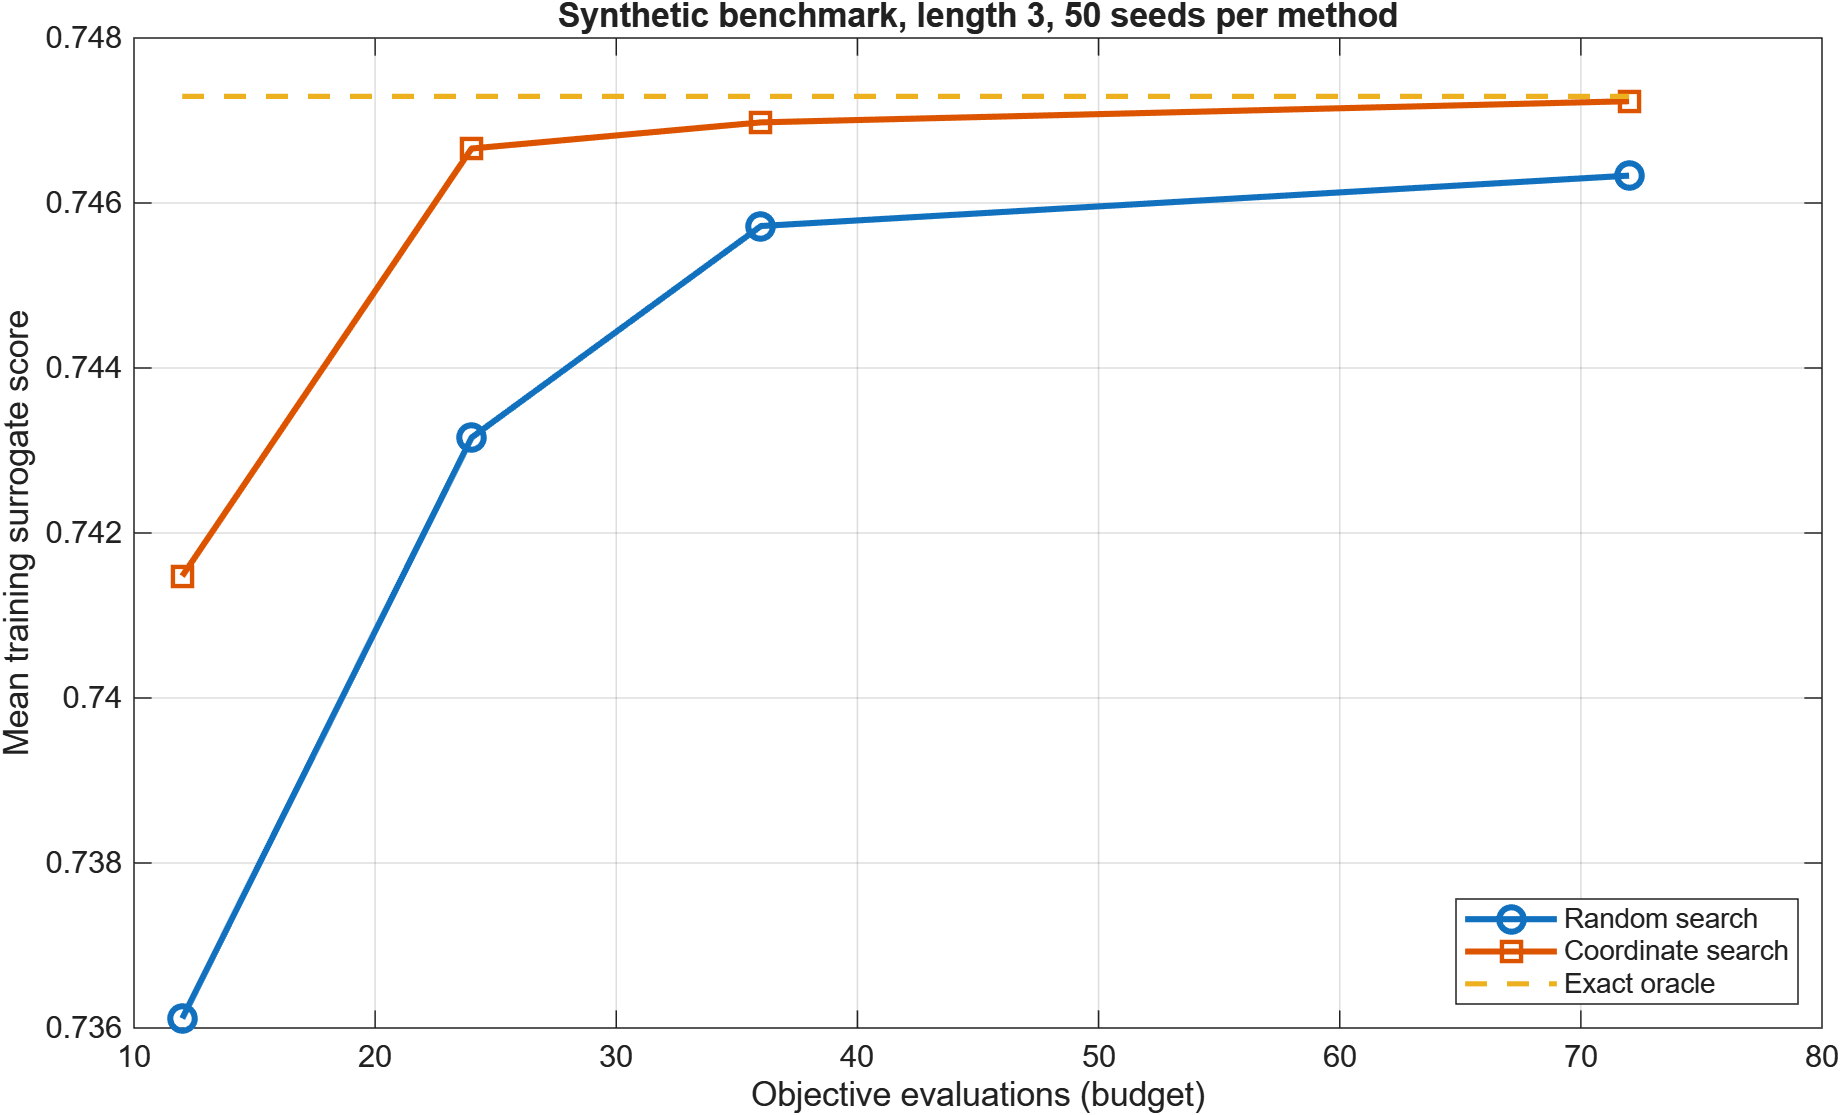
\includegraphics[width=.93\linewidth]{../evidence/native-matlab/matlab_score_budget.png}
\caption{Native MATLAB rendering of recorded synthetic training scores for three-token prompts across score-call budgets, with the exhaustive oracle as a fixed reference.}\label{fig:matlab-budget}
\end{figure}
The oracle line is not a third heuristic. It records the best of all $6^3=216$ possibilities, requiring exhaustive evaluation beyond the budget of the search methods. Both heuristic curves are based on fifty algorithmic seeds for each budget. Since each search retains its best observation, increasing its budget cannot lower its own best score in a given run. That monotonicity does not guarantee monotonic performance on independent held-out tasks.

\section{Regret across prompt lengths}
\begin{figure}[htbp]\centering
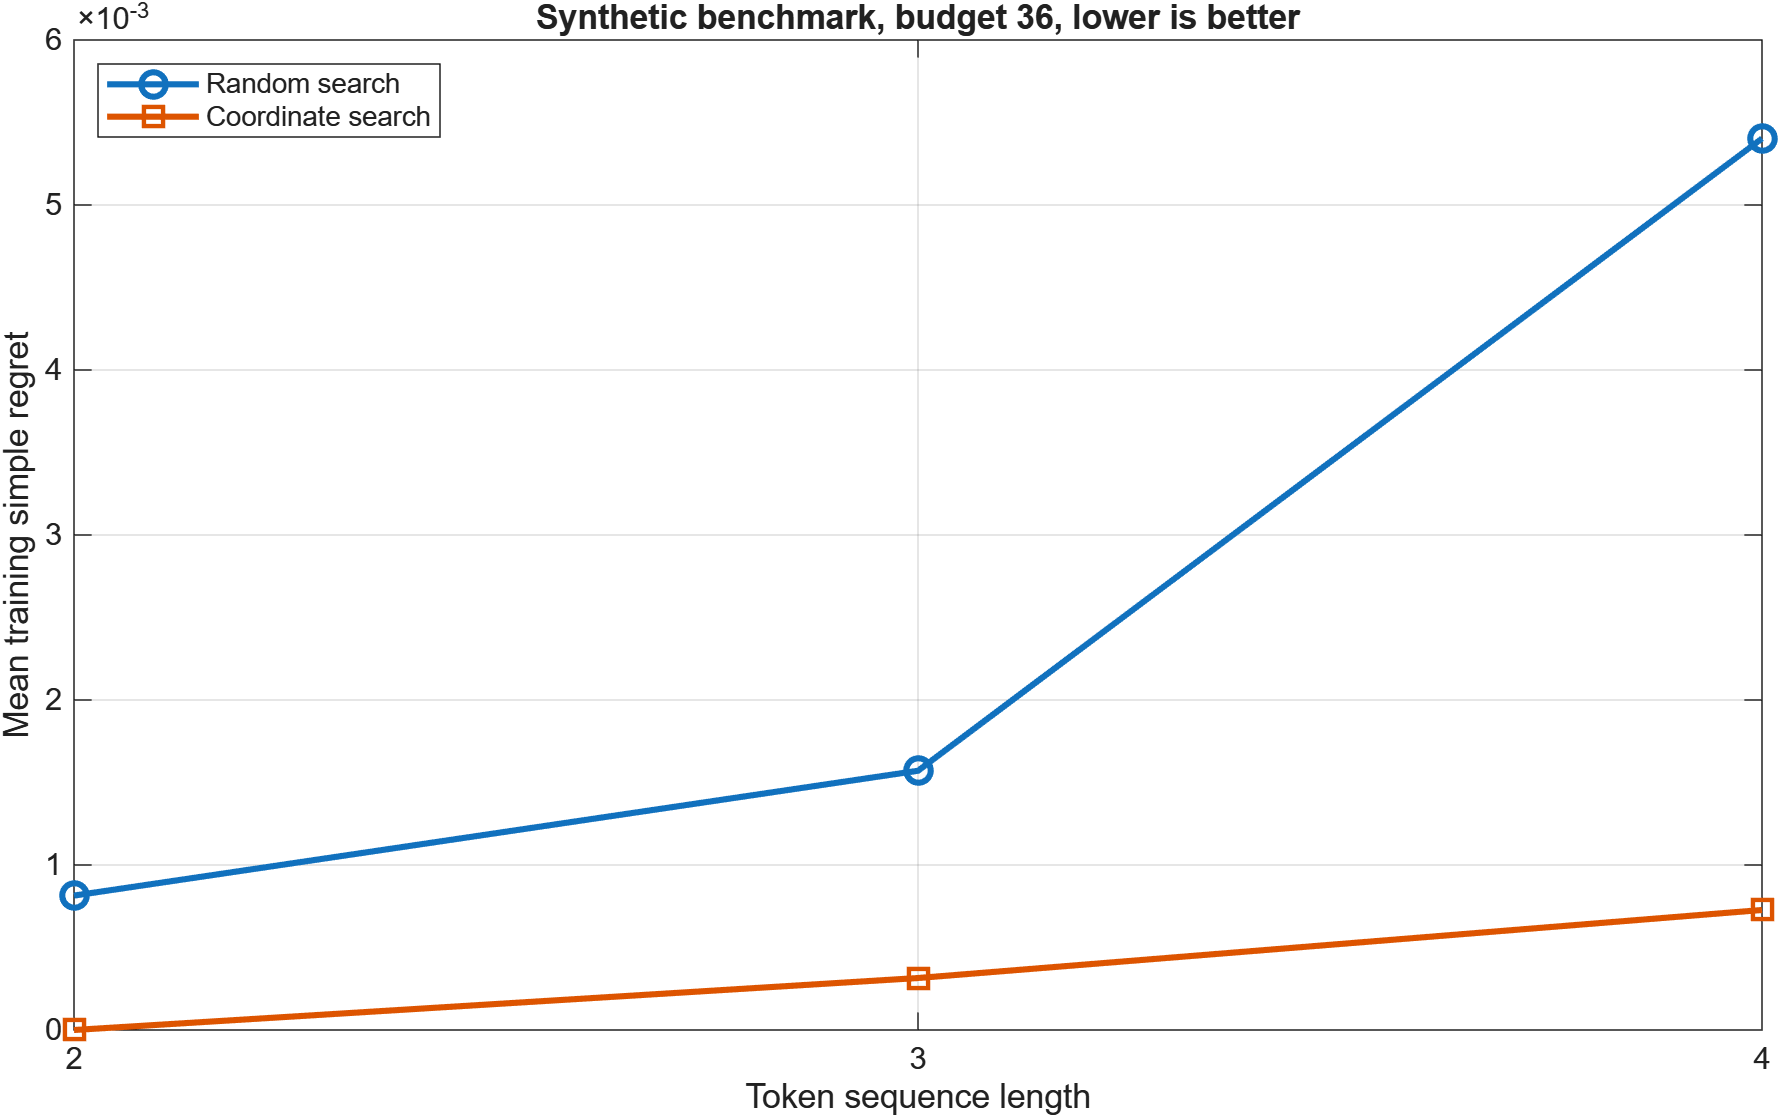
\includegraphics[width=.93\linewidth]{../evidence/native-matlab/matlab_regret_length.png}
\caption{Mean simple regret at a fixed budget of 36 scorer calls, comparing prompt lengths two, three and four. Lower regret means a smaller gap to the length-specific exact oracle.}\label{fig:matlab-regret}
\end{figure}
For each length $m$, simple regret is defined as $r_B=J_m^*-J(\hat p_B)$. The optimal score $J_m^*$ is recomputed separately for that length, so regret is interpretable within a length but is not an identical task across lengths. In particular, length changes both the number of candidate sequences and the weighted embedding geometry of the surrogate.

\section{Held-out scores and model-selection limitation}
\begin{figure}[htbp]\centering
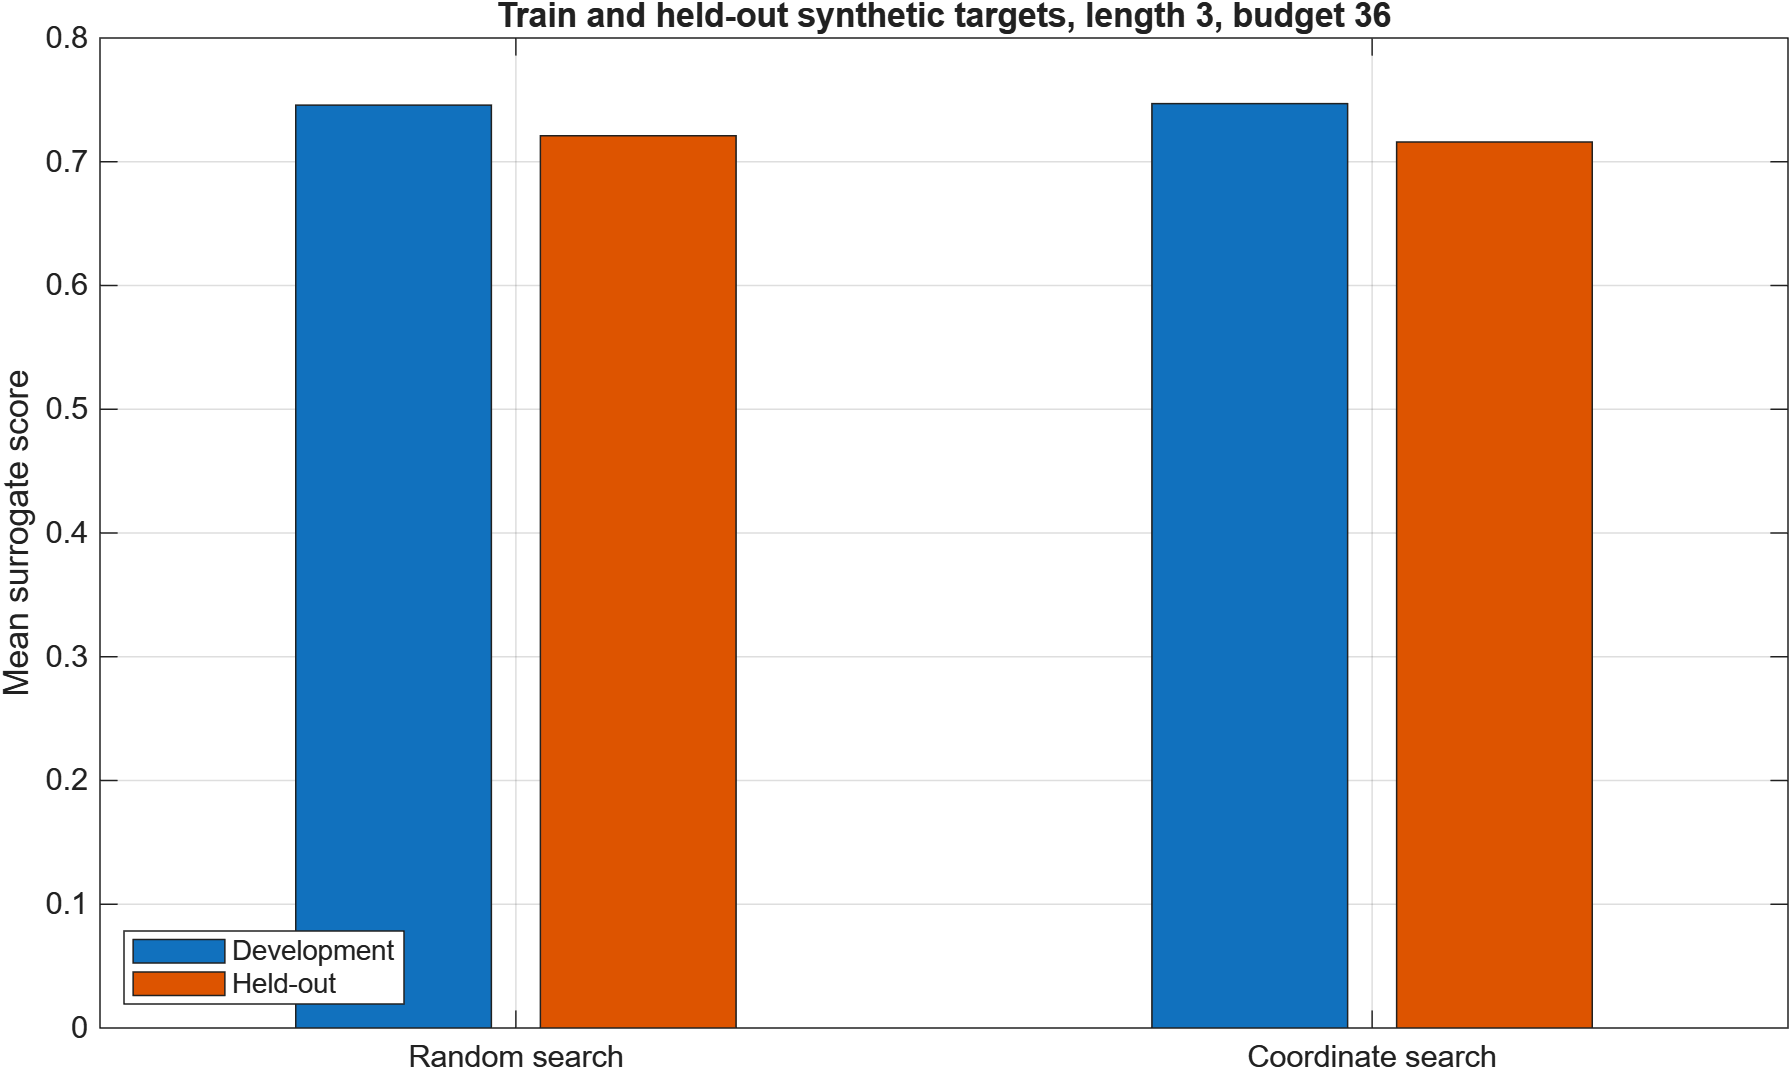
\includegraphics[width=.93\linewidth]{../evidence/native-matlab/matlab_train_holdout.png}
\caption{Development and held-out synthetic mean scores for the 3-token, 36-call condition. The held-out targets are fixed vectors, not task-labelled samples generated by an LLM.}\label{fig:matlab-heldout}
\end{figure}
A higher development objective need not imply a higher held-out objective. These target vectors were specified in code and do not constitute an externally sampled data distribution. The held-out comparison checks the analysis pipeline and illustrates the need for separation of prompt selection and evaluation. It is not an estimate of generalization to real prompts.

\section{Paired-seed differences and uncertainty}
\begin{figure}[htbp]\centering
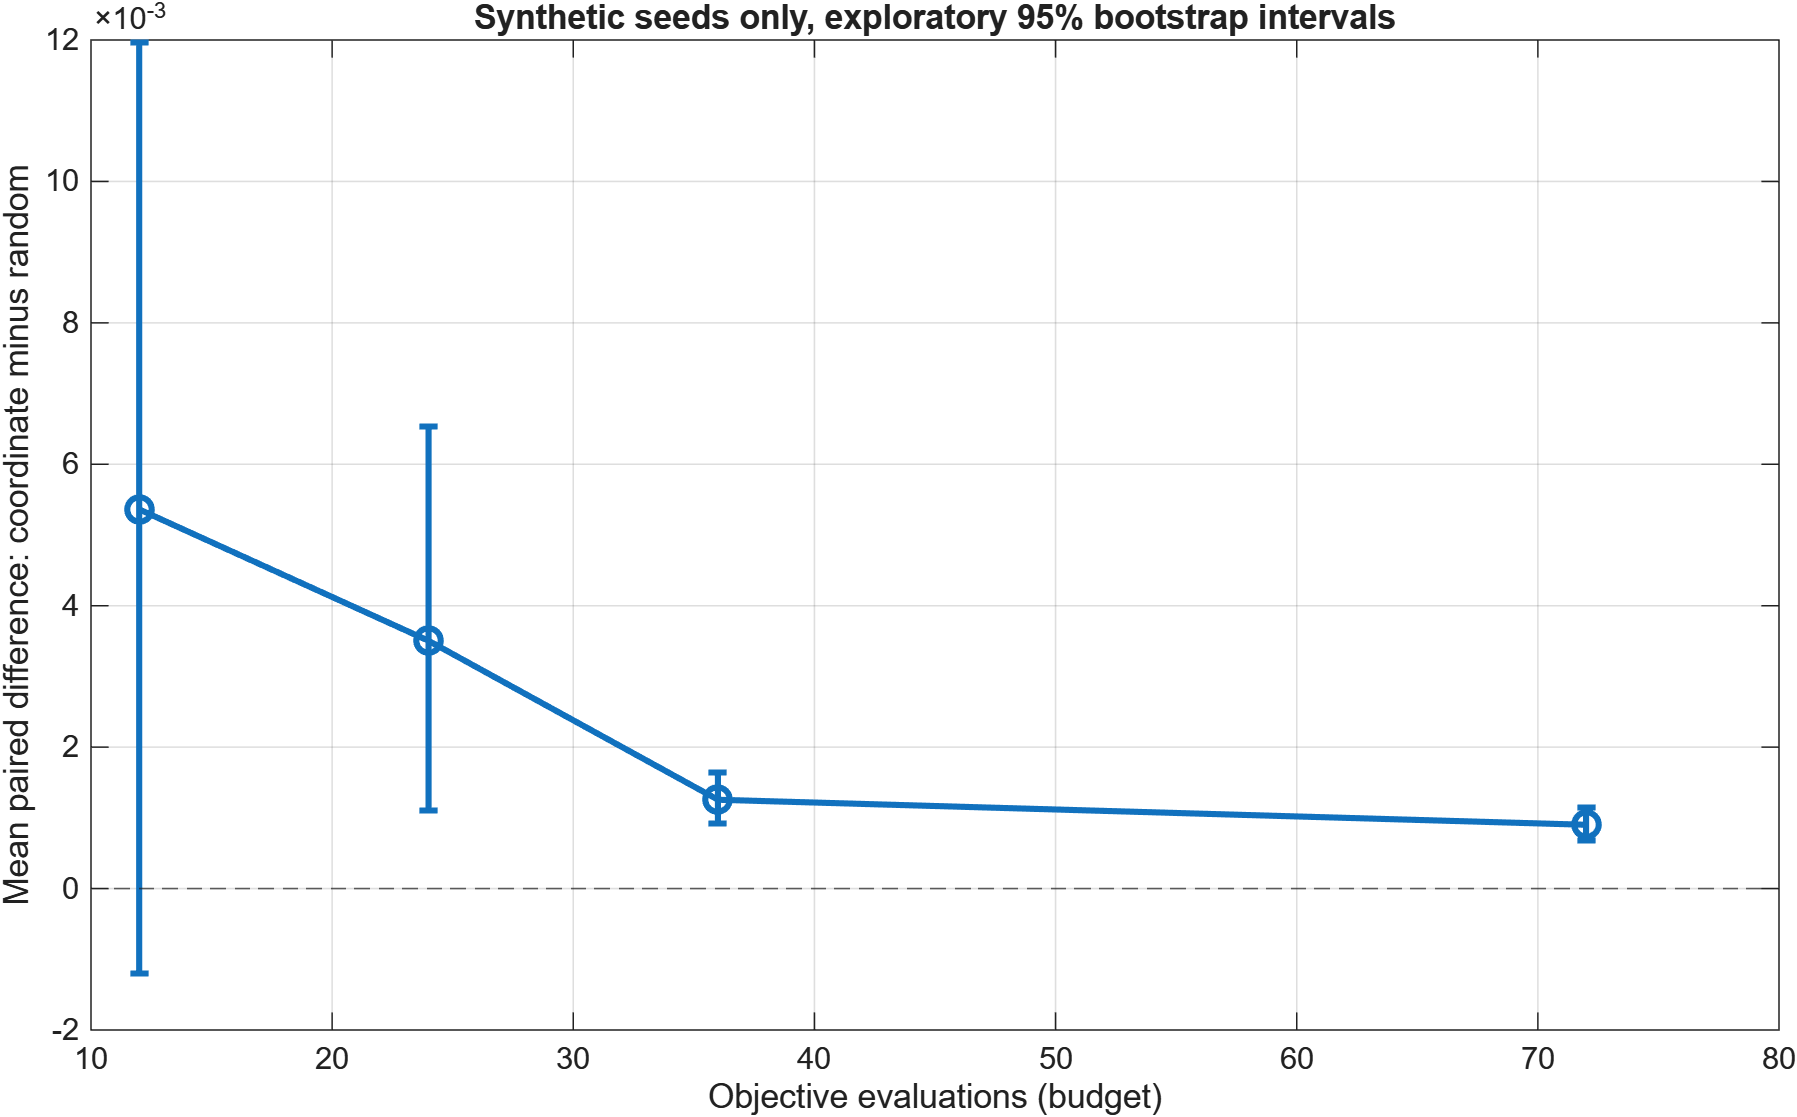
\includegraphics[width=.93\linewidth]{../evidence/native-matlab/matlab_paired_difference.png}
\caption{Exploratory paired-seed mean differences for three-token prompts. Error bars are percentile bootstrap intervals computed over algorithmic seed pairs. They are not confidence intervals for a population of LLM tasks.}\label{fig:matlab-pairs}
\end{figure}
For seed index $s$ and evaluation budget $B$ define $D_{s,B}=J(\hat p^{\rm coordinate}_{s,B})-J(\hat p^{\rm random}_{s,B})$. The plotted point is $50^{-1}\sum_{s=0}^{49}D_{s,B}$. The intervals resample the fifty paired differences with replacement. Because the same synthetic objective is reused across all seeds and budgets, treating these as independent examples of natural-language tasks would be incorrect. Exploratory $p$-values are not adjusted for testing twelve configurations, so statistical claims should be limited to this controlled computational setup.

\section{Reproducing the MATLAB figures}
\begin{lstlisting}[language=bash]
# From the project root, first verify the synthetic record.
python3 -m unittest discover -s tests -v
# In MATLAB, change directory to the project root and call:
# addpath('matlab')
# generate_thesis_figures(pwd)
\end{lstlisting}
Running the MATLAB script from the repository root generates four PNG files under \texttt{tex/figures}; the separately committed native render evidence used in this chapter is retained under \texttt{evidence/native-matlab/} with its render log. To rebuild the dissertation, run XeLaTeX twice in the \texttt{tex} directory. A visual comparison against the older Python-rendered copies remains future validation if cross-renderer parity is claimed.

\chapter{Prospective Real-Model Evaluation Protocol}
\section{Status: proposed, not run}
No real-model calls, licensed datasets, live latency recordings or human ratings are included in this thesis milestone. This chapter states a testable, pre-declared protocol for later execution, not an experiment with missing results quietly filled in by the surrogate.

\section{Tasks and splits}
Select two to three reproducible tasks with objective automatic scoring, for example label classification with a fixed label set and structured extraction with deterministic schema validation. Record dataset source, license, annotation quality, disjoint development and test partitions, evaluation language and exact sample IDs. Use development samples for prompt selection. Evaluate the final selected prompt on the held-out test partition only once per preregistered run. If a pilot test requires altering the protocol, label it exploratory rather than reporting it as a confirmatory replication.

\section{Model configuration}
Record model identifier and revision, tokenizer revision, context length, instruction hierarchy, decoding temperature, top-$p$, seed if supported, maximum output tokens, retry policy and dates of execution. A hosted API may change independently of the thesis source, record the returned version and provider release notes where available. Do not mix outputs from different revisions under one model name.

\section{Baselines and fairness}
Compare at least a fixed author-written instruction, uniform random candidate selection and coordinate-style editing under matched development-evaluation calls. When a gradient-based method is available, give its additional gradient computation a separately reported cost. Report search wall time and actual input and output token totals in addition to call counts. The same validation and normalization rules must be applied to every method.

\section{Scoring and uncertainty}
For classification or exact-format extraction, choose one primary score before evaluating. Exact match is defined by $\ind[\hat y_i=y_i]$ under pre-declared normalization, validity rate is $n^{-1}\sum_i\ind[C(\hat y_i)=1]$. Accuracy should not be used as a synonym for a surrogate probability. When examples are paired across prompt methods, use paired intervals or an appropriate paired resampling procedure. Report per-task scores and failure categories, an aggregate alone may conceal a method that fails on one task.

\section{Offline results evaluator}
\texttt{src/score\_outputs.py} accepts JSON Lines records that must contain a task ID, example ID, model identifier, prompt identifier, reference string, prediction string, schema-validity Boolean, token counts and latency. It calculates grouped exact-match rates, validity rates and mean usage. It \emph{does not} call a model, fabricate observations, verify the provenance of externally supplied records or assert a result without input data. That boundary is intentional. A later evaluation should preserve raw response files, prompt templates, hashes, model parameters and a signed run manifest.

\section{Ethics and reproducibility checks}
Review dataset licenses, use non-sensitive input data, avoid including private prompts or personal records in a public repository, and consult the supervisor on ethics requirements before collecting human judgments. Reproducibility means another researcher can obtain the same software behavior and inspect raw evidence, it does not imply access to a proprietary model version is guaranteed indefinitely.

\chapter{Discussion, Validity and Limitations}
\section{Answer to RQ1}
The decision variable for a fixed-length textual prompt is a tuple in a Cartesian power of a finite set. The downstream computation is defined through real-valued embeddings and a neural conditional distribution. A joint objective can refer to both domains, but ordinary derivatives apply only after a continuous representation has been specified. This distinction is a mathematically precise interpretation, consistent with the submitted article and the prompting literature.

\section{Answer to RQ2}
The project derives the candidate count $N^m$, explicit surrogate gradients, a Lipschitz bound, enumeration complexity, the exact random-optimum probability and expected-best formula. The executable tests check representative numerical consequences. These are formal or computational facts under stated definitions, not empirical laws of language-model behavior.

\section{Answer to RQ3}
Under the fixed six-symbol surrogate, coordinate search achieves lower mean training regret than uniform random search in the reported three-token, thirty-six-evaluation condition. Both methods were given the same number of score calls, exact oracles were available because the space was small. The small target vectors, smooth logistic objective, greedy neighborhood and seeded restarts all shape the result. Performance on a different surrogate or task cannot be inferred without new data.

\section{Answer to RQ4}
Real-model conclusions require task-aligned, licensed data, held-out sets, versioned models, exact prompt definitions, repeated measurements, matched search budgets, failure analyses, and uncertainty appropriate to the experimental design. The offline evaluation interface and prospective protocol specify these requirements but do not satisfy them on their own.

\section{Threats to internal validity}
The synthetic scorer has no tokenizer, contextual attention, memory, autoregressive decoding, semantic representations or instruction hierarchy. The chosen vectors are subjective fixtures. Because the scoring function is smooth and low-dimensional, one-coordinate substitutions may be substantially easier to optimize than natural-language instructions. The source code's seed control and exact oracle make internal numerical checks possible but do not remove these modelling assumptions.

\section{Threats to external validity}
A six-symbol vocabulary and prompt lengths below five do not represent realistic LLM input spaces. Moreover, the token labels resemble English words but are merely names for hard-coded vectors. The toy objective can illustrate calculus and search, it cannot establish that one of these words is a superior prompt in any real model. Results cannot be generalized to multilingual prompts, safety-sensitive systems, user preferences or changing deployed models.

\section{Statistical caution}
Fifty seeds are deterministic repetitions of randomized algorithms on one fixed function, not fifty independently sampled real-world tasks. Bootstrap intervals describe dispersion under this seed design only. Statistical significance in this setting would not answer whether a method improves LLM accuracy in deployment. If a future LLM study uses prompt selection on a development set, choosing hypotheses after inspecting the held-out test would invalidate its confirmatory interpretation.

\section{Reproducibility and originality}
The code and mathematical results are inspectable. Some formulas are standard: neither the softmax derivative nor the coupon-style random-hit probability is claimed as a novel discovery. The thesis's specific contribution is their explicit integration into a controlled, reproducible prompt-search study, with exact-score baselines and an evidence register. Related research should be cited as foundational rather than framed as absent from the literature.

\chapter{Conclusion and Remaining Submission Requirements}
The dissertation has developed the core mathematical claim of the submitted short article into a formal, executable investigation. The completed component establishes an exact finite optimization benchmark, checks differentiable surrogate calculations, compares budget-matched search procedures and exposes results in CSV, JSON and XeLaTeX. This supports an undergraduate conclusion about \emph{methodology}: one can study the discrete selection of prompts against a continuous evaluation function without conflating the two mathematical operations.

The work is not yet an institutionally finished thesis. A final departmental submission should incorporate the supervisor's feedback, the approved thesis template and assessment criteria, a verified bibliography and - if the approved project requires empirical performance claims - actual held-out LLM runs under the protocol of Chapter 8. No numeric outcome from those future experiments is predicted or invented here. Further legitimate extensions include robust optimization under distribution shift, uncertainty from stochastic decoding, and multi-objective search balancing success, validation failures and compute cost.

\appendix
\chapter{Reproduction Guide}
\section{Local environment}
The validated implementation uses Python 3.13 locally and is designed for Python 3.10 or later without third-party packages for the experiment itself. The manuscript uses XeLaTeX, a TeX Gyre font and PGFPlots. An internet connection or LLM account is unnecessary for the synthetic stage.
\begin{lstlisting}[language=bash]
python3 -m unittest discover -s tests -v
python3 src/experiment.py
python3 src/make_tables.py
python3 src/paired_analysis.py
python3 src/gradient_audit.py
python3 src/landscape_audit.py
cd tex
xelatex -halt-on-error -interaction=nonstopmode thesis.tex
xelatex -halt-on-error -interaction=nonstopmode thesis.tex
\end{lstlisting}
The generated dataset contains $1200$ CSV rows and a JSON file containing twelve configurations. The manuscript results tables are generated from that JSON, edits to the Python objective require regeneration before the PDF build.

\section{Real-model records (not included)}
To score external model outputs after they actually exist, prepare one JSON object per line with the fields:\par
\begin{lstlisting}
{"id":"ex1","task":"classification","model":"versioned-model-id",
 "prompt_id":"baseline","expected":"yes","prediction":"yes",
 "output_valid":true,"input_tokens":24,"output_tokens":2,
 "latency_ms":130.0}
\end{lstlisting}
The example above is a \emph{schema illustration}, not experimental data. Run
\begin{lstlisting}[language=bash]
python3 src/score_outputs.py --input actual_predictions.jsonl \
  --output actual_scores.json
\end{lstlisting}
The input records and model invocation process are the experimenter's responsibility.

\chapter{Evidence Register and Completion Criteria}
\small
\begin{longtable}{p{0.28\textwidth}p{0.27\textwidth}p{0.35\textwidth}}
\toprule Component&Current status&Required verification for final submission\\\midrule\endhead
Submitted October 2026 short article&Author-provided theoretical preprint&Confirm citation/relationship and institutional reuse policy\\
Discrete/continuous definitions&Written and mathematically inspectable&Supervisor review of notation and scope\\
Analytical gradients and search formulas&Derived in Chapter 4&Independent mathematical proofreading\\
Exhaustive finite oracles&Executed in synthetic benchmark&Recompute from pinned repository commit\\
Heuristic comparisons&1200 synthetic records&Confirm CI and inspect code for hidden scoring calls\\
Unit tests&27 passed locally&Verify on GitHub CI after push\\
Exhaustive landscape and gradient audits&Per-state gradient rankings and discrete terminal-state JSON for $m\in\{2,3,4\}$&Re-run both standard-library Python audit generators and review objective/tolerance assumptions\\
MATLAB figure generation&Native MATLAB R2026b render log and four PNGs committed in \texttt{evidence/native-matlab/}&Compare against the earlier Python renders only if visual parity is claimed\\
Reproducible XeLaTeX draft&Generated from tracked source&Check compiled PDF and department formatting\\
Real LLM task data and inference&\textbf{Not performed}&Select datasets, acquire approvals, execute held-out protocol\\
Human assessments&\textbf{Not performed}&Only if needed and institutionally approved\\
Supervisor and academic acceptance&\textbf{Not confirmed}&Document review and final sign-off\\\bottomrule
\end{longtable}
\normalsize

\begin{thebibliography}{99}
\bibitem{brown2020} Brown, T. B., et al. (2020). Language Models are Few-Shot Learners. \emph{Advances in Neural Information Processing Systems}, 33, 1877--1901.
\bibitem{vaswani2017} Vaswani, A., et al. (2017). Attention Is All You Need. \emph{Advances in Neural Information Processing Systems}, 30.
\bibitem{lester2021} Lester, B., Al-Rfou, R., and Constant, N. (2021). The Power of Scale for Parameter-Efficient Prompt Tuning. \emph{EMNLP}, 3045--3059. \href{https://doi.org/10.18653/v1/2021.emnlp-main.243}{doi:10.18653/v1/2021.emnlp-main.243}.
\bibitem{shin2020} Shin, T., Razeghi, Y., Logan IV, R. L., Wallace, E., and Singh, S. (2020). AutoPrompt: Eliciting Knowledge from Language Models with Automatically Generated Prompts. \emph{EMNLP}, 4222--4235. \href{https://doi.org/10.18653/v1/2020.emnlp-main.346}{doi:10.18653/v1/2020.emnlp-main.346}.
\bibitem{lu2022} Lu, Y., Bartolo, M., Moore, A., Riedel, S., and Stenetorp, P. (2022). Fantastically Ordered Prompts and Where to Find Them: Overcoming Few-Shot Prompt Order Sensitivity. \emph{ACL}, 8086--8098. \href{https://doi.org/10.18653/v1/2022.acl-long.556}{doi:10.18653/v1/2022.acl-long.556}.
\bibitem{zhao2021} Zhao, Z., Wallace, E., Feng, S., Klein, D., and Singh, S. (2021). Calibrate Before Use: Improving Few-Shot Performance of Language Models. \emph{ICML}, 12697--12706.
\bibitem{zhou2023} Zhou, Y., et al. (2023). Large Language Models Are Human-Level Prompt Engineers. \emph{ICLR}.
\bibitem{liu2023} Liu, P., et al. (2023). Pre-train, Prompt, and Predict: A Systematic Survey of Prompting Methods in Natural Language Processing. \emph{ACM Computing Surveys}, 55(9). \href{https://doi.org/10.1145/3560815}{doi:10.1145/3560815}.
\bibitem{ahmad2026} Ahmad, R., et al. (2026). A Society of AI Scientists. \emph{alphaXiv} preprint, submitted November 19, 2026. \href{https://www.alphaxiv.org/abs/2611.society-ai-scientists}{alphaXiv:2611.society-ai-scientists}.
\bibitem{nadiotis2026} Nadiotis, C. (2026). \emph{Prompt Engineering as a Discrete-Continuous Optimization Problem: A Mathematical Perspective Using Discrete Mathematics and Calculus}. Author-provided short article, submitted in October 2026, publication status not independently verified.
\end{thebibliography}
\end{document}
